\subsection{Использование инспектора свойств}
\label{sec:manual:inspector_manual}

Компонент инспектор свойств представляет из себя панель инструментов, показанную на рисунке~\ref{sec:manual:inspector}.

Навигация по вкладкам <<DATA>>, <<STYLES>> и <<CODE>> осуществляется путем нажатия на нужную. На каждой странице есть элементы, которые пользователь может сворачивать и разворачивать.

На рисунке~\ref{sec:manual:inspector} показано содержимое вкладки <<STYLES>>. Здесь в элеиенте <<Formatting>> отображаются свойства последнего выделенного компонента.

Кнопки внизу содержимого элемента <<Formatting>> осуществляют добавление компоненту свойства (кнопка <<ADD PROPERTY>>) и удаление компонента (и всех его дочерних элементов, если такие присутствуют) с грид разметки (кнопка <<DELETE COMPONENT>>).

\begin{figure}[ht]
  \centering
    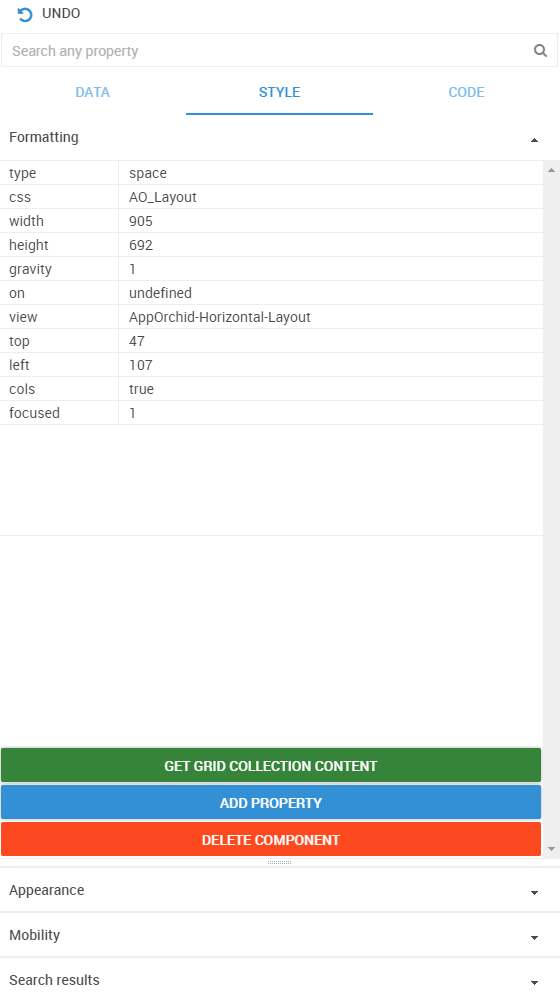
\includegraphics[scale=0.5]{inspector.png}
    \caption{Внешний вид инспектора свойств}
    \label{sec:manual:inspector}
\end{figure}
  
Вверху компонента присутствует кнопка <<UNDO>>, отменяющая последнее произошедшее действие. Прямо под ней расположена строка поиска свойств. Поиск осуществляется путем ввода нужного значения в поле для ввода и нажатия кнопки Enter. После нажатия будет произведен поиск свойств по ключу и значению, все результаты поиска будут выведены в элементе <<Search results>>, который развернется автоматически.

Результат вышеуказанных действий показан на рисунке~\ref{sec:manual:inspector_search_manual}.\pagebreak

\begin{figure}[ht]
  \centering
    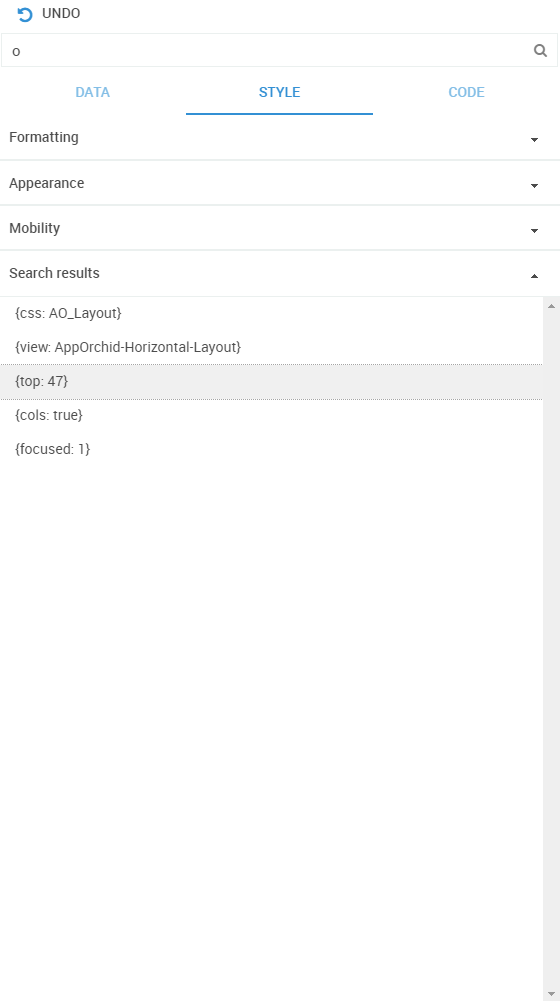
\includegraphics[scale=0.5]{inspector_search_manual.png}
    \caption{Отображение результатов поиска в инспекторе свойств}
    \label{sec:manual:inspector_search_manual}
\end{figure}

Результаты поиска предоставляются на основании проведения операции проверки вхождения введенной строки в ключи и значения свойств компонента. 

При нажатии на элемент списка будет открыта соответствующая вкладка со свойствами и выбранное свойство автоматически будет выбрано для редактирования, как показано на рисунке~\ref{sec:manual:inspector_search_manual_results}.\pagebreak

\begin{figure}[ht]
  \centering
    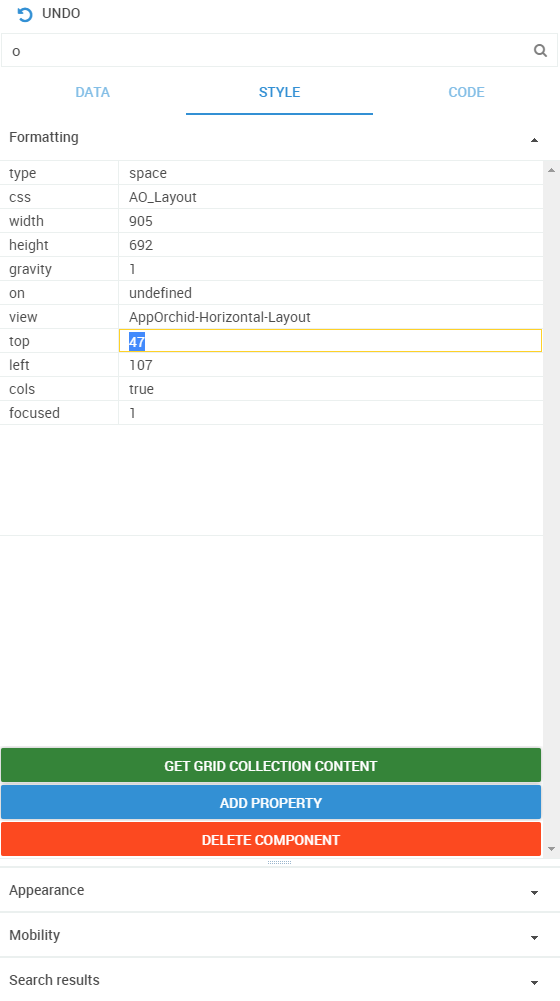
\includegraphics[scale=0.5]{inspector_search_manual_results.png}
    \caption{Редактирование свойств}
    \label{sec:manual:inspector_search_manual_results}
\end{figure}

Во вкладке <<CODE>> будет отображаться код объекта конфигурации последнего выделенного компонента. Показанный на рисунке~\ref{sec:manual:inspector_code} код является кодом компонента библиотеки Webix. В данном месте не отображается код дочерних компонентов - это сделано для большей читаемости.
\pagebreak

\begin{figure}[ht]
  \centering
    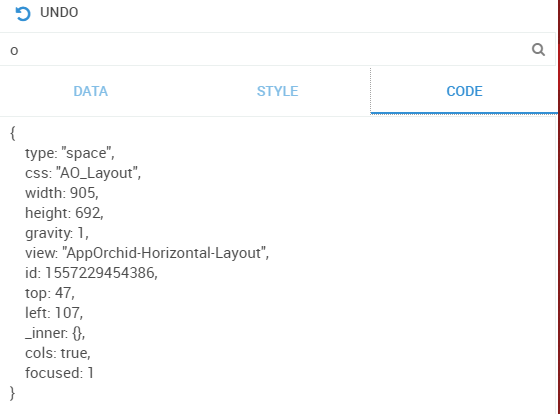
\includegraphics[scale=0.5]{inspector_code.png}
    \caption{Внешний вид вкладки <<CODE>>}
    \label{sec:manual:inspector_code}
\end{figure}